\section{Buck Converter Battery Charging Simulation (High Ratings)} % This will display as 5.3 Buck Converter Battery Charging Simulation

\subsection{System Parameters} % This becomes 5.3.1
The simulation model consists of a DC-link buck converter supplying a series $RC$ load, which models the electrical behavior of a battery.

\begin{table}[h!]
\centering
\caption{Simulation Configuration Parameters}
\label{tab:parameters}
\begin{tabular}{ll}
\toprule
\textbf{Parameter} & \textbf{Value} \\ 
\midrule
Input Voltage ($V_{dc}$) & $600\text{ V}$ \\
Filter Inductor ($L$) & $30\text{ mH}$ \\
Output Capacitor ($C_{out}$) & $200\ \mu\text{F}$ \\
Equivalent Load Resistance ($R$) & $1\ \Omega$ \\
Equivalent Load Capacitance ($C$) & $0.5\text{ F}$ \\
\bottomrule
\end{tabular}
\end{table}

\subsection{Control Strategy} % This becomes 5.3.2
The system implements a dual-mode closed-loop PID control strategy to replicate a standard Constant Current / Constant Voltage (CC/CV) battery charging profile.

\begin{itemize}
    \item \textbf{Mode 1: Constant Current (CC) Mode}
    \begin{itemize}
        \item \textbf{Condition:} Measured voltage $V_{out} < V_{ref}$ ($570\text{ V}$).
        \item \textbf{Operation:} The current loop PID regulates the charging current to a fixed reference of $20\text{ A}$.
    \end{itemize}
    
    \item \textbf{Mode 2: Constant Voltage (CV) Mode}
    \begin{itemize}
        \item \textbf{Condition:} Measured voltage $V_{out} \ge V_{ref}$ ($570\text{ V}$).
        \item \textbf{Operation:} Control switches to the voltage loop PID, clamping the output at $570\text{ V}$ while the current naturally decays.
    \end{itemize}
\end{itemize}

\begin{figure}[h!]
    \centering
    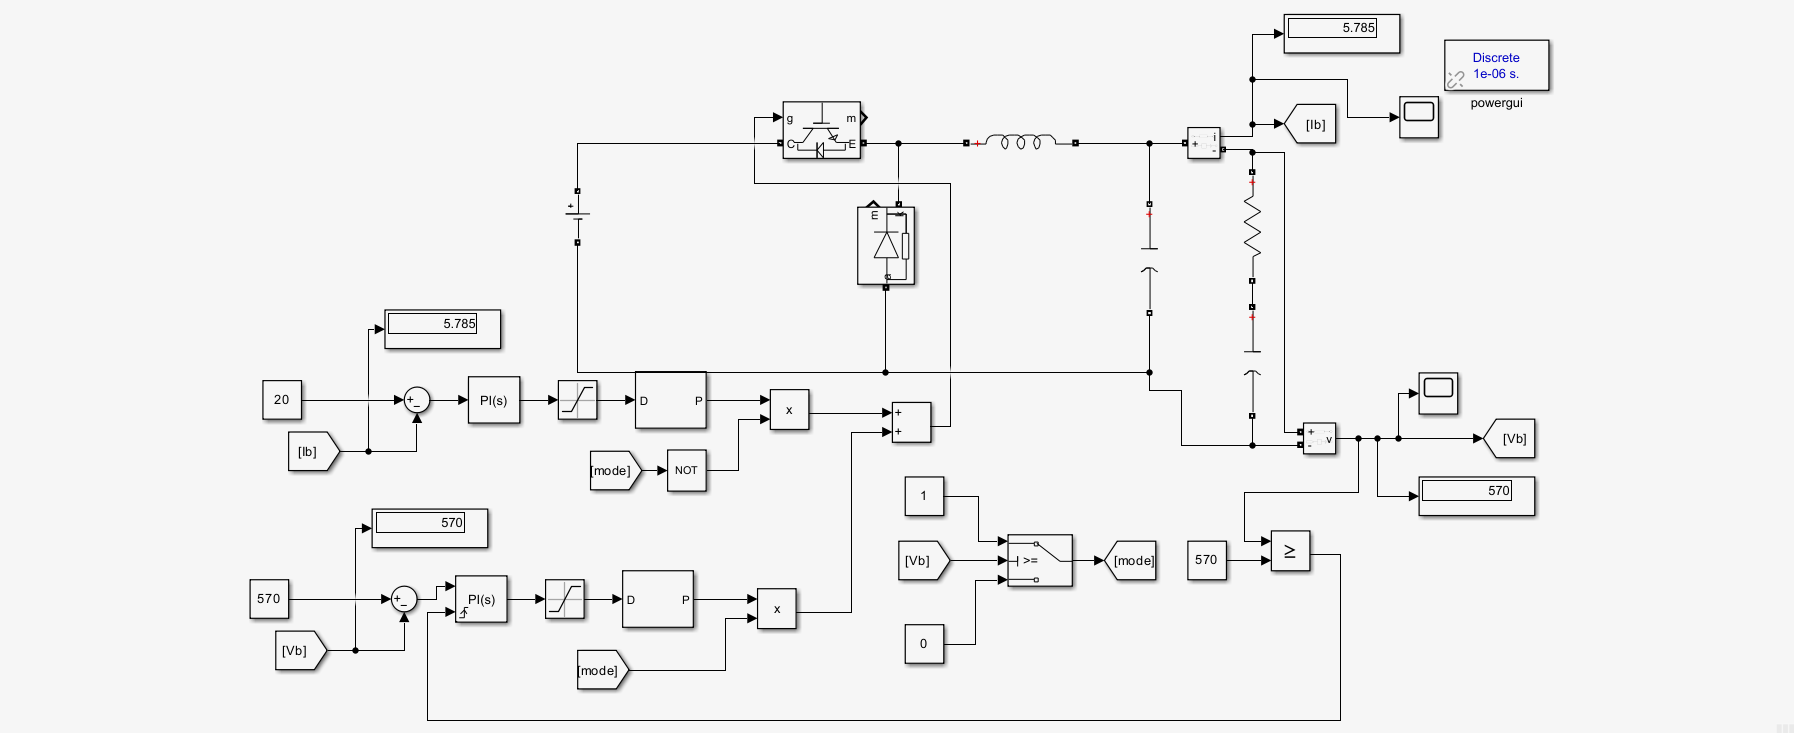
\includegraphics[width=0.8\textwidth]{Figures/volt.png} 
    \caption{MATLAB/Simulink Control Mode Boundary Analysis}
    \label{fig:control_boundary}
\end{figure}

\subsection{Simulation Results \& Discussion} % This becomes 5.3.3

\paragraph{Phase Analysis}
\begin{itemize}
    \item \textbf{Transient Phase (CC Mode):} Initially, the battery voltage is below $570\text{ V}$. The current PID loop successfully regulates the charging current to $20\text{ A}$, causing the battery capacitor to charge linearly.
\end{itemize}

\begin{figure}[h!]
    \centering
    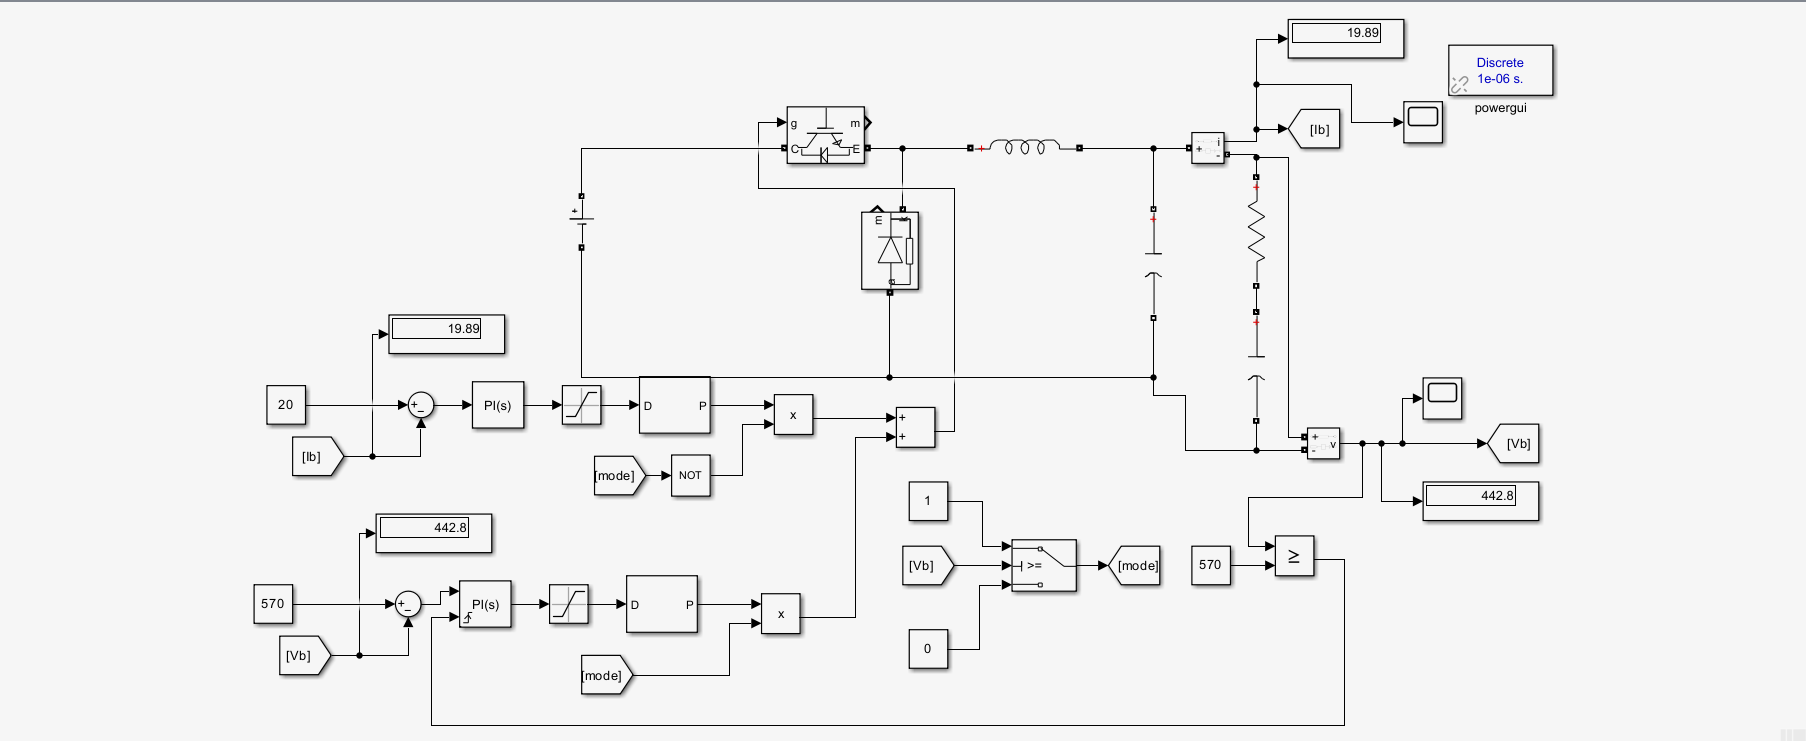
\includegraphics[width=0.8\textwidth]{Figures/current.png} 
    \caption{MATLAB/Simulink Current Response Waveform}
    \label{fig:current_waveform}
\end{figure}

\begin{itemize}
    \item \textbf{Transition Phase:} Once the battery voltage reaches the $570\text{ V}$ threshold, the control logic smoothly transitions from current control to voltage control.
    \item \textbf{Steady-State Phase (CV Mode):} The voltage PID loop stabilizes the output at $570\text{ V}$. As the battery approaches full charge, the current exponentially decays toward zero, preventing overcharging.
\end{itemize}

\paragraph{Scope Observations}
\begin{itemize}
    \item \textbf{Current Scope ($I$):} Shows a constant $20\text{ A}$ plateau during the CC phase, followed by a sharp exponential decay toward $0\text{ A}$ once CV mode is activated.
    
    \item \textbf{Voltage Scope ($V$):} Displays a linear voltage rise during the CC phase, which smoothly flattens out and stabilizes precisely at the $570\text{ V}$ threshold as the controller switches modes.
\end{itemize}

\begin{figure}[h!]
    \centering
    \begin{minipage}{0.48\textwidth}
        \centering
        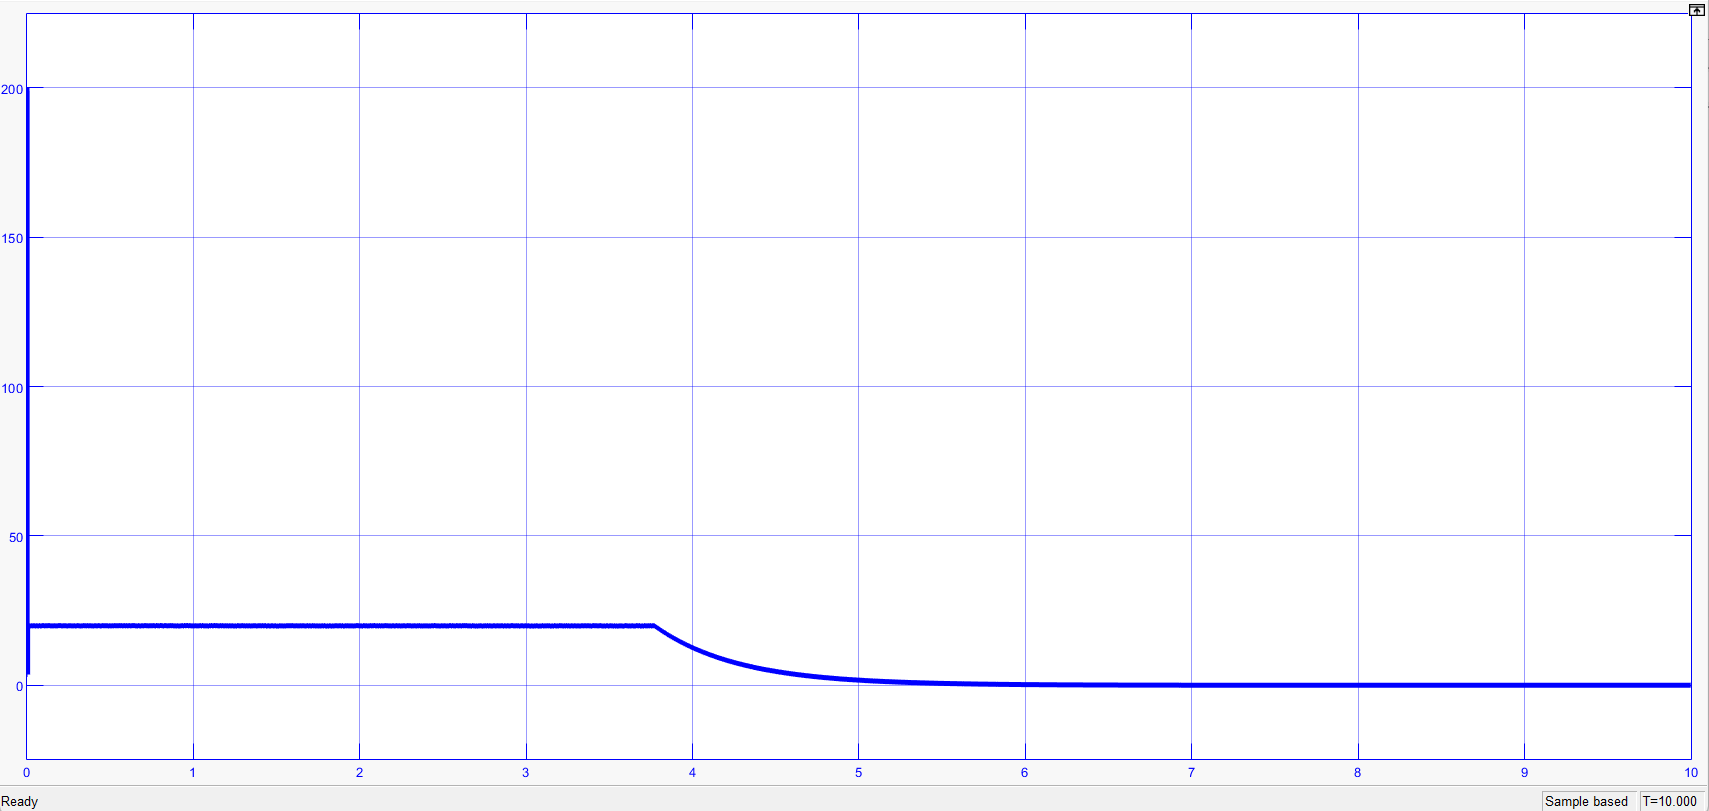
\includegraphics[width=\textwidth]{Figures/current scope.png} 
        \caption{Charging Current ($I$)}
        \label{fig:current_scope}
    \end{minipage}
    \hfill
    \begin{minipage}{0.48\textwidth}
        \centering
        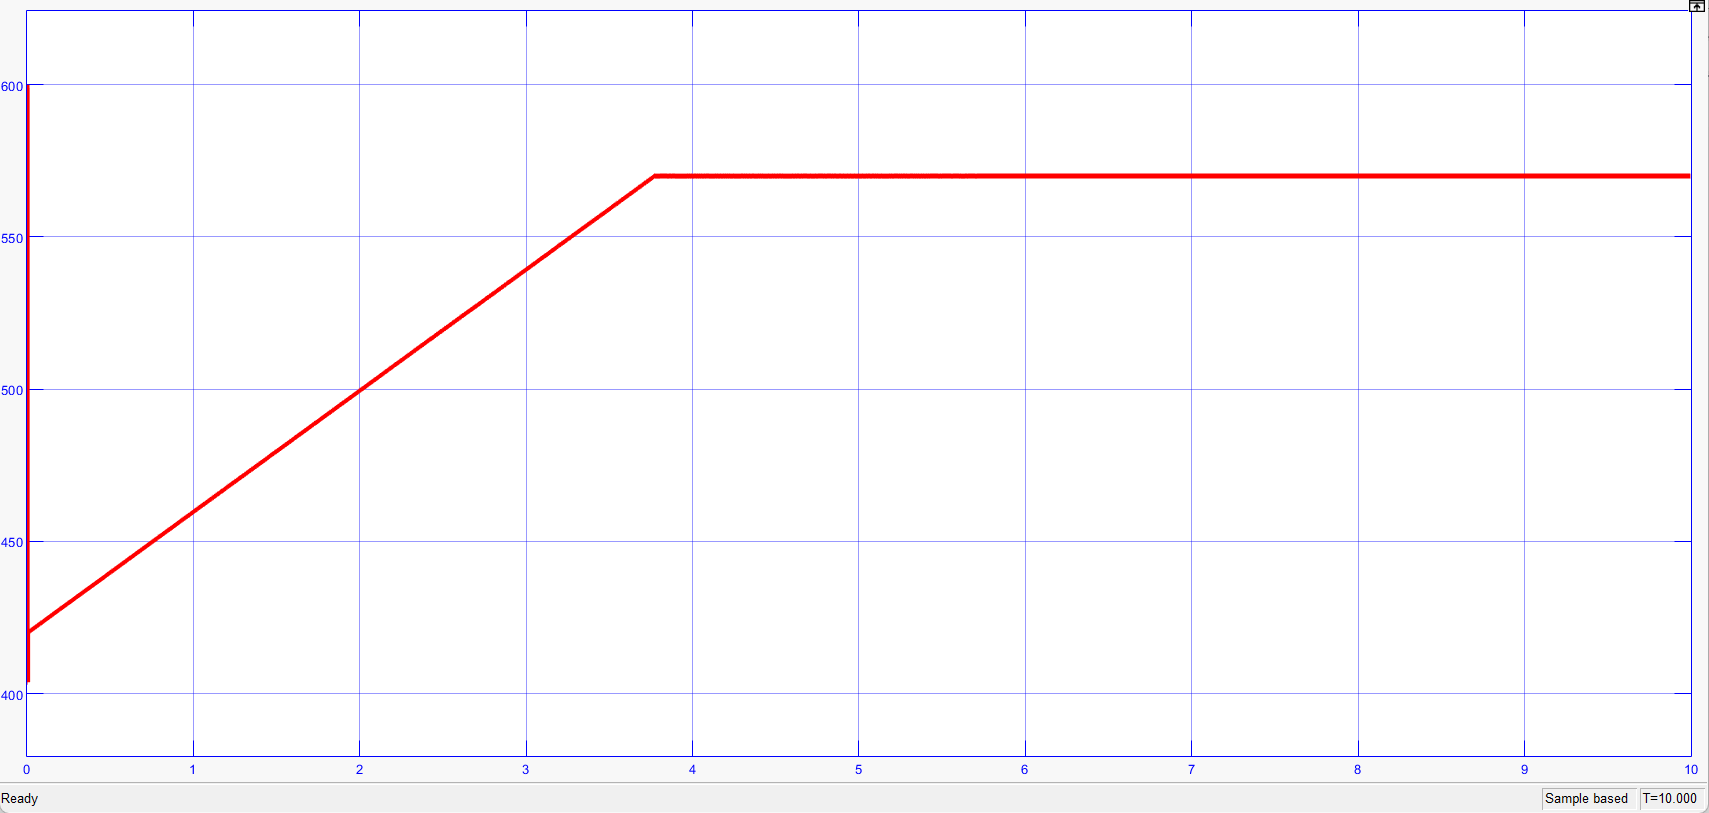
\includegraphics[width=\textwidth]{Figures/volt scope.png}
        \caption{Battery Voltage ($V$)}
        \label{fig:voltage_scope}
    \end{minipage}
\end{figure}
\newpage
\subsection{Conclusion} % This becomes 5.3.4
The closed-loop buck converter successfully demonstrates automated CC/CV battery charging. The transition between the current-controlled phase ($20\text{ A}$) and the voltage-controlled phase ($570\text{ V}$) is stable, ensuring safe and efficient energy transfer to the $RC$ battery model.
